%%%%%%%%%%%%%%%%%%%%%%%%%%%%%%%%%%%%%%%%%%%%%%%%%%%%%%%%%%%%%%%%%%%%%%
% LaTeX Example: Project Report
%
% Source: http://www.howtotex.com
%
% Feel free to distribute this example, but please keep the referral
% to howtotex.com
% Date: March 2011 
% 
%%%%%%%%%%%%%%%%%%%%%%%%%%%%%%%%%%%%%%%%%%%%%%%%%%%%%%%%%%%%%%%%%%%%%%
% How to use writeLaTeX: 
%
% You edit the source code here on the left, and the preview on the
% right shows you the result within a few seconds.
%
% Bookmark this page and share the URL with your co-authors. They can
% edit at the same time!
%
% You can upload figures, bibliographies, custom classes and
% styles using the files menu.
%
% If you're new to LaTeX, the wikibook is a great place to start:
% http://en.wikibooks.org/wiki/LaTeX
%
%%%%%%%%%%%%%%%%%%%%%%%%%%%%%%%%%%%%%%%%%%%%%%%%%%%%%%%%%%%%%%%%%%%%%%
% Edit the title below to update the display in My Documents
%\title{Project Report}
%
%%% Preamble
\documentclass[paper=a4, fontsize=11pt]{scrartcl}
\usepackage[T1]{fontenc}
\usepackage{fourier}

\usepackage[english]{babel}															% English language/hyphenation
\usepackage[protrusion=true,expansion=true]{microtype}	
\usepackage{amsmath,amsfonts,amsthm} % Math packages
\usepackage[pdftex]{graphicx}	
\usepackage{url}
\usepackage{titlesec}
\usepackage{mathtools}
\usepackage{enumitem}
%\usepackage{lstlisting}


%%% Custom headers/footers (fancyhdr package)
\usepackage{fancyhdr}
\pagestyle{fancyplain}
\fancyhead{}											% No page header
\fancyfoot[L]{}											% Empty 
\fancyfoot[C]{}											% Empty
\fancyfoot[R]{\thepage}									% Pagenumbering
\renewcommand{\headrulewidth}{0pt}			% Remove header underlines
\renewcommand{\footrulewidth}{0pt}				% Remove footer underlines
\setlength{\headheight}{13.6pt}
\usepackage[margin=0.5in]{geometry}

%%% Equation and float numbering
\numberwithin{equation}{section}		% Equationnumbering: section.eq#
\numberwithin{figure}{section}			% Figurenumbering: section.fig#
\numberwithin{table}{section}				% Tablenumbering: section.tab#

%% Section Format
\titleformat*{\section}{\LARGE\bfseries}
\titleformat*{\subsection}{\Large\bfseries}
\titleformat*{\subsubsection}{\large\bfseries}
\titleformat*{\paragraph}{\large\bfseries}
\titleformat*{\subparagraph}{\large\bfseries}

\DeclarePairedDelimiter{\ceil}{\lceil}{\rceil}

%%% Maketitle metadata
\newcommand{\horrule}[1]{\rule{\linewidth}{#1}} 	% Horizontal rule

\title{
		%\vspace{-1in} 	
		\usefont{OT1}{bch}{b}{n}
		\normalfont \normalsize \textsc{University of Purdue\\
      Data Communication and Computer Networks\\
      CS 53600 Spring 2020} \\ [25pt]
		\horrule{0.5pt} \\[0.4cm]
		\huge Assignment 5\\
		\horrule{2pt} \\[0.5cm]
}
\author{
		\normalfont\normalsize Pedro da Costa Abreu Júnior\\ [-5pt]
    \normalsize Student ID 0030878383\\[-5pt]
    \normalsize \today
}
\date{}


%%% Begin document
\begin{document}
\maketitle

\section*{Problem 1}
\begin{center}
\begin{tabular}{c c c c c c c c}
       &     & D(z) & D(y) & D(v) & D(w) & D(t) & D(u) \\
  Step & N'  & p(z) & p(y) & p(v) & p(w) & p(t) & p(u) \\
  0    & X   & 8,X  & 6,X  & 3,X  & 6,X  & $$\infty$$ & $$\infty$$ \\
  \hline
  1    & Xv  & 8,X  & 6,X  &      & 6,X  & 7,v & 6,v \\
  \hline
  2    & Xvy & 8,X  &      &      & 6,X  & 7,v & 6,v \\
  \hline
  3    & Xvyw & 8,X  &      &      &     & 7,v & 6,v \\
  \hline
  4    & Xvywu & 8,X  &      &      &     & 7,v &    \\
  \hline
  5    & Xvywut & 8,X  &      &      &     &    &    \\
  \hline
  6    & Xvywut &      &      &      &     &    &    \\
  \hline
\end{tabular}
\end{center}

\section*{Problem 2}
B and C does not share to X and W that they are connected, leading to the following views of the network:

\begin{figure}[h]
  \label{fig:w_view}
  \caption{W view of the topology}
  \centering
  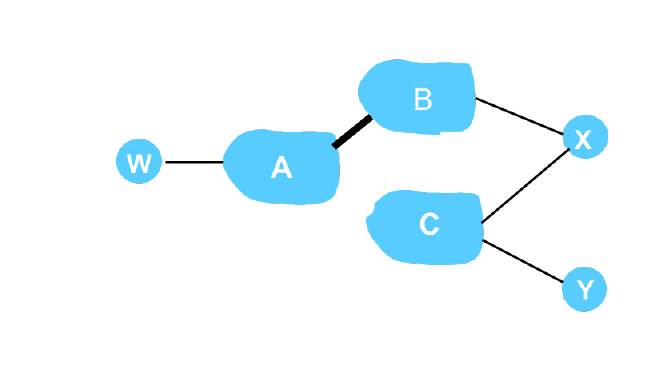
\includegraphics[width=0.5\textwidth]{x_view}
\end{figure}
\begin{figure}[h]
  \label{fig:x_view}
  \caption{X view of the topology}
  \centering
  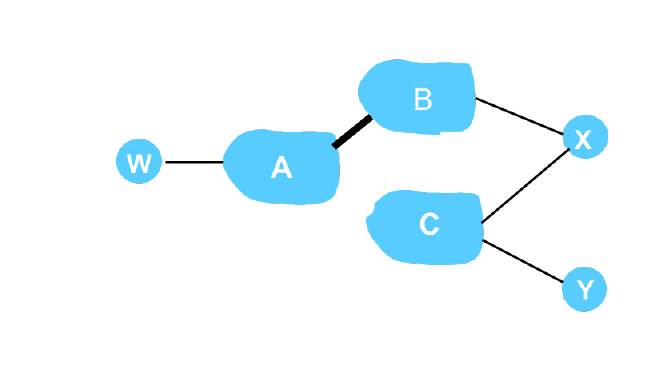
\includegraphics[width=0.5\textwidth]{x_view}
\end{figure}

\section*{Problem3}
\begin{enumerate}[label=\alph*)]
  \item eBGP
  \item OSPF + iBGP
  \item eBGP
  \item IS-IS + iBGP
  \item l1, because it is the nearest router to take the package to another AS.
  \item l2, because it is the nearest router to take the package to another AS.
\end{itemize}


%%% End document
\end{document}

%%% Local Variables:
%%% mode: latex
%%% TeX-master: t
%%% End:
